
\documentclass[9pt]{IEEEtran}

% basic
\usepackage[slovene]{babel}
\usepackage{graphicx,epstopdf,fancyhdr,amsmath,amsthm,amssymb,url,array,textcomp,svg,listings,hyperref,xcolor,colortbl,float,gensymb,longtable,supertabular,multicol,placeins}
\usepackage{diagbox}
 % `sumniki' in names
\usepackage[utf8x]{inputenc}
\usepackage{multirow}
\usepackage{makecell}

 % search and copy for `sumniki'
\usepackage[T1]{fontenc}
\usepackage{lmodern}
\input{glyphtounicode}
\pdfgentounicode=1

% tidy figures
\graphicspath{{./figures/}}
\DeclareGraphicsExtensions{.pdf,.png,.jpg,.eps}

% correct bad hyphenation here
\hyphenation{op-tical net-works semi-conduc-tor trig-gs}

% ============================================================================================

\title{\vspace{0ex} %
% TITLE IN HERE:
Izločanje očesnih artefaktov z uporabo postopka s
pasovno prepustnim filtrom (Butterworth) in
pragovno metodo
\\ \large{2. seminarska naloga}\\ \normalsize{Komunikacija človek-računalnik 2021/22, Fakulteta za računalništvo in informatiko, Univerza v Ljubljani}}
\author{ %
% AUTHOR IN HERE:
Žiga~Kleine
\vspace{-4.0ex}
}

% ============================================================================================

\begin{document}

\maketitle

\begin{abstract}

V poročilu bomo predstavili implementacijo in delovanje programa za izločevanje artefaktov, ki v EEG posnetkih nastanejo predvsem med utripanjem oči in predstavljajo neželen šum na omenjenih posnetkih. Problema smo se lotili tako, da smo signal najprej dvosmerno filtrirali z pasovno prepustnim Butterworth filtrom, da smo izničili visokofrekvenčne šume in lezenje ničelnega nivoja, nato pa smo iz filtriranega signala poskusili izrezati neželene artefakte tako, da smo iz signala odstranili dele, katerih amplituda presega določen prag. Na koncu smo signal z odstranjenimi artefakti primerjali z začetnim signalom.


\end{abstract}

\section{Uvod}

Implementacijo vmesnika, s katerim lahko s pomočjo možganske aktivnosti nadzorujemo računalnik, lahko razdelimo na 5 smiselnih faz. Te faze so: zajemanje signalov, preobdelava ali čiščenje signalov, izločanje značilk, klasifikacija in interakcija z računalnikom.

Pri tej seminarski smo se posvetili drugi prej omenjeni fazi, čiščenju signalov. Ko z elektrodami zajemamo električne signale na površini možganov, se v teh signalih zelo pogosto pojavljajo šumi, ki niso povezani z možgansko aktivnostjo. Te šume lahko razdelimo v štiri glavne kategorije: šume, ki jih povzroči EEG oprema, zunanje električne motnje, šume, ki jih povzročijo žice elektrod, in šume, ki jih povzroči pacient ~\cite{gupta1996preprocessing}. Pri tej seminarski nalogi se bomo posvetili predvsem šumom, ki jih povzroči pacient. Med najintenzivnejšimi šumi, še posebno pri elektrodah na sprednjem delu glave, so namreč šumi, ki jih povzročajo obrazne mišice med mežikanjem in premikanjem oči. Te bomo poskušali iz signala izločiti s pragovno metodo, ostale pa bomo poskušili čim bolj izničiti z uporabo pasovno prepustnega filtra.

\section{Metode}

Program za izločanje očesnih artefaktov z uporabo postopka s pasovno prepustnim filtrom in pragovno metodo smo implementirali v programskem jeziku MATLAB. Najprej smo s portala Physionet s pomočjo programskega paketa wfdb pridobili EEG posnetke s prisotnimi očesnimi artefakti. Pridobljene signale smo najprej filtrirali s pasovno prepustnim Butterworthovim filtrom, nato smo poiskali ustrezen prag, in nazadnje še na podlagi praga iz signala še odstranili zaznane artefakte ~\cite{ochoa2002eeg}.

\begin{figure}[!htb]
\centering
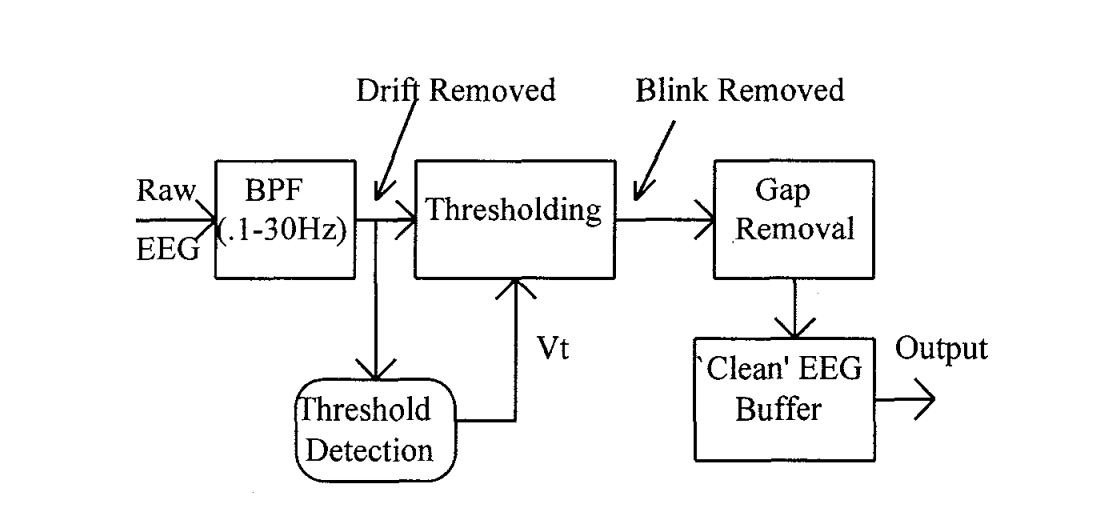
\includegraphics[width=1\columnwidth]{shema.png}
\caption[c1]{ Shema programa za izločanje artefaktov ~\cite{gupta1996preprocessing}. }
\label{fig_1}
\end{figure}

\subsection{Priprava in izris signalov}

Signale smo pridobili iz opdprte podatkovne baze biomedicinskih signalov Physionet, specifično iz podatkovne baze EEG posnetkov z imenom EEG Motor Movement/Imagery Dataset \cite{goldberger2000physiobank, schalk2004bci2000}. Pri procesiranju signalov smo si pomagali s programskim paketom wfdb, ki je na voljo tudi v programskem okolju MATLAB.

\subsection{Dvosmerno filtriranje signala}

Izbrani signal smo nato dvosmerno filtrirali s pasovno prepustnim Butterworthovim filtrom. Filter smo implementirali s pomočjo vgrajene MATLAB funkcije $butter$, ki nam generira koeficienta za želen Butterworth filter. Za potrebe projetka smo generirali pasovno prepustmi filter 4. reda z spodnjo mejo $0.1 Hz$ in zgornjo mejo $30 Hz$. Na ta način smo eliminirali tako počasno lezenje ničelnega nivoja, kot ostale morebitne neželene frekvence v signalu. Da smo izničili fazni zamik signala, smo signal najprej filtrirali, ga obrnili, ga nato spet filtrirali, in ga nazadnje spet obrnili. Na ta način se je fazni zamik filtra izničil.

\subsection{Določanje praga za razpoznavo artefaktov}

Za določenje praga za detekcijo in kasnejše izločanje artefaktov smo si pomagali z implementacijo, opisano v članku ~\cite{gupta1996preprocessing}. Tu so prag določili iz začetnega dela vhodnega signala tako, da so signal najprej  razdelili na 30 kosov (mi smo ga razdelili na 60), od katerih je bil vsak dolg 125 vzorcev.  Za vsakega od kosov so izračunali povprečje ~\ref{eq1} in standardno deviacijo ~\ref{eq2} absolutne vrednosti signala. Končni prag pa so nato dobili tako, da so vzeli povprečni vrednosti kosa z najmanjšo deviacijo $\mu_{\sigma\_min}$ in kosa z največjo deviacijo $\mu_{\sigma\_max}$, in ju povprečili ~\ref{eq3}. Kos signala z največjo standardno deviacijo naj bi predstavljal del signala, kjer je prisoten artefakt in kos z najmanjšo deviacijo naj bo predstavljal normalen signal. 

\begin{equation} \label{eq1}
\mu_j = \dfrac{\sum_{i=1}^{N} abs(x_j(i))}{N}
\end{equation}

\begin{equation} \label{eq2}
\sigma_j = \sqrt{\dfrac{\sum_{i=1}^{N} (abs(x_j(i)) - \mu_j)^2}{N}}
\end{equation}

\begin{equation} \label{eq3}
threshold = \dfrac{\mu_{\sigma\_max} + \mu_{\sigma\_min}}{2}
\end{equation}

\subsection{Odstranjevanje zaznanih artefaktov} 
 
Po tem ko smo signal uspešno filtrirali in mu določili prag, smo se z zanko sprehodili čez celoten signal in iz njega odstranili vse zaznane artefakte. Artefakt smo zaznali vsakič, ko je amplituda signala presegla prag. Ko smo artefakt zaznali, smo ga odstranili najprej tako, da smo N vzorcev signala v okolici zaznanega artefakta najprej nastavili na 0, nato pa smo te dele še odstranili iz signala. Spremenljivki N smo z opazovanjem artefaktov v signalu določili vrednost 6.

\section{Rezultati}

Delovanje naše implementacije smo testirali predvsem s signali elektrod na sprednjem delu glave, kjer so očesni artefakti najintenzivnejši. 

Na slikah lahko vidimo signal iz eegmidb z imenom $S001R03.edf$, in sicer specifično signal elektrode čelnega režnja elektrode 22 z imenom $F_{P1}$ na sliki \ref{fig2}, in signal elektrode 24 z imenom $F_{P2}$ na sliki \ref{fig3}. Na vrhu obeh slik vidimo vhodni signal, na sredini je signal po filtriranju z pasovno prepustnim filtrom, spodaj pa signal po izločanju artefaktov. Na signalih po izločanju artefaktov se jasno vidi, da je bil del signala, ki je vseboval artefakte, izločen. Z omenjeno metodo za določanje praga smo na signalu elektrode 22 dobili prag vrednosti $81.9869$ in na signalu elektrode 24 prag vrednosti $78.4011$.

\begin{figure}[!htb]
\centering
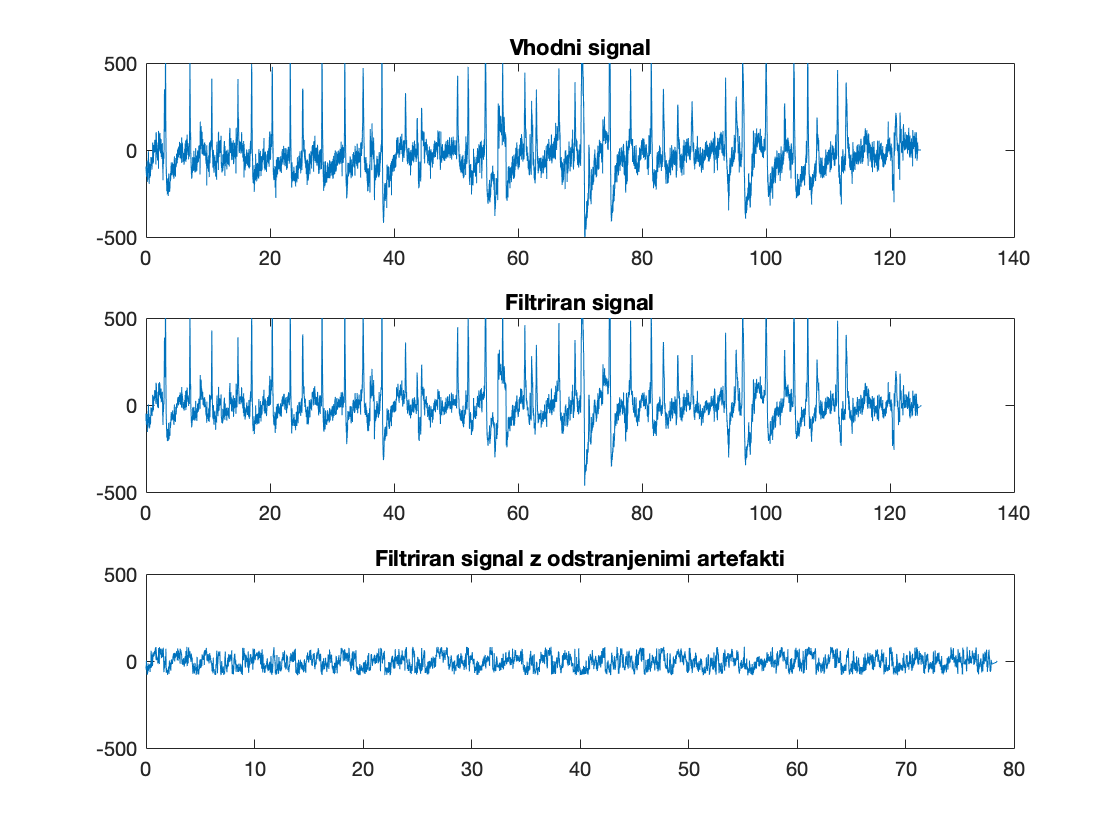
\includegraphics[width=1\columnwidth]{results22.png}
\caption[c1]{ Signal elektrode 22 z imenom $F_{P1}$.  }
\label{fig_2}
\end{figure}

\begin{figure}[!htb]
\centering
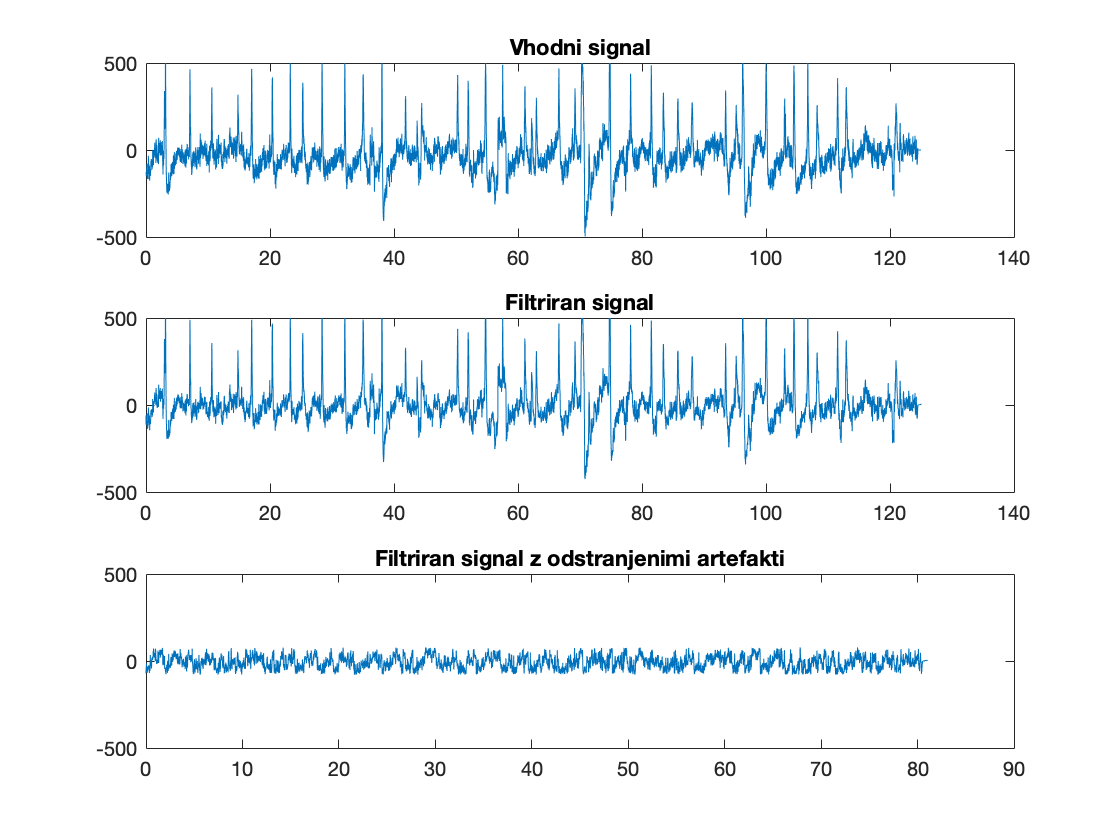
\includegraphics[width=1\columnwidth]{results24.png}
\caption[c1]{ Signal elektrode 24 z imenom $F_{P2}$.}
\label{fig_3}
\end{figure}


\section{Diskusija}

Opisana metoda je kljub svoji preprosti implementaciji precej učinkovita pri odstranjevanju večjih artefaktov iz šumnih EEG signalov. Pri trenutni implementaciji se bodo težave začele pojavljati, če je v posnetku prisotnih zelo veliko mežikov. Tak signal namreč naša implementacija močno skrajša iz njega odstrani morebitne uporabne informacije.

Algoritem bi lahko izboljšali tako, da bi na primer dinamično nastavljali dolžino artefakta, ki ga režemo iz signala, saj trenutno uporabljamo fiksno dolžino, za katero ni nujno da odraža dolžino artefaktov v vhodnem signalu.


\bibliographystyle{IEEEtran}
\bibliography{bibliography}

\end{document}


 %\ref{table2}:
% \begin{table}[!htb]
% \centering
% \begin{tabular}{|c|c|} \hline
% Nn & true positive \\ \hline
% Nv & false negative \\ \hline
% Vn & false positive \\ \hline
% Vv & true negative  \\ \hline
% \end{tabular}
% \label{table2}
% \end{table}